

\chapter{多摄像头系统的时间同步}

\section{本章引言}

对于摄像头拍摄时间的检测,其主要目的是为了验证对多摄像头系统同步工作的准确性。在能够获得摄像头准确拍摄时间的基础上,本章主要介绍对多摄像头系统进行时间同步的具体过程。其中包括在实际应用过程当中出现的几个问题,这些问题虽然表面看起来并不重要,有时候却会对系统同步造成较大影响,并且由于在日常摄像头的应用中这些问题并不常见,很容易对其忽视影响同步结果。同时本章还介绍了系统同步的方法,包括软硬件的系统配置,同步过程,同步检验,同步优化等。

\section{同步过程中存在的几个问题}

\subsection{果冻效应}

果冻效应(the Jello Effect)是由于摄像头自身特性所引起的一种曝光效果。对于卷帘快门摄像头来说,其在拍摄过程中感光传感器是从第一行开始到最后一行逐行打开,逐行开始曝光的。所以从第一行开始曝光到整个感光传感器全部打开,整个开始曝光会持续很短的一段时间。在日常应用中,这种卷帘快门快门打开时间很短,对拍照造成的影响很小。但是当使用卷帘快门摄像头拍摄高速运动的物体时,由于整个感光传感器内各行开始曝光的时间不同,拍摄到的物体就会出现倾斜、摇摆或者部分曝光等现象。对于摄像头的曝光时间来说,是从第一行快门打开开始计算,因此最后几行快门的总曝光时间,就需要在总曝光时间基础上,减去摄像头卷帘快门的打开时间。如图~\ref{jelly}所示即为一种典型的果冻效应的图像。

如果此摄像头不存在果冻效应,整个感光传感器同时开始曝光,那么在传感器曝光过程中,螺旋桨从上至下扫过整幅图像,就可以拍摄到连续的移动画面。而由于果冻效应的影响,摄像头的快门由上至下逐行打开,当第一行快门打开时,螺旋桨已经运动到第一行感光传感器所对应的视野范围内的下半部分,所以拍摄到螺旋桨的图像只存在于此视野范围内的下半部分,上半部分并没有螺旋桨图像。而当第二行快门打开时,螺旋桨又已经运动到第二行感光传感器所对应的视野范围内的下半部分,再次拍摄到一部分存在一部分不存在的螺旋桨图像。以此类推,这也就导致拍摄到的螺旋桨的图像并不连续,造成如图所示的效果。只有螺旋桨的运动速度足够快,才能使得每次新打开的感光传感器视野内都只有一部分能够拍摄到螺旋桨的图像。在普通拍摄中,拍摄对象运动速度较慢,是不会出现这种现象的。

\begin{figure}[h] 
  \centering
  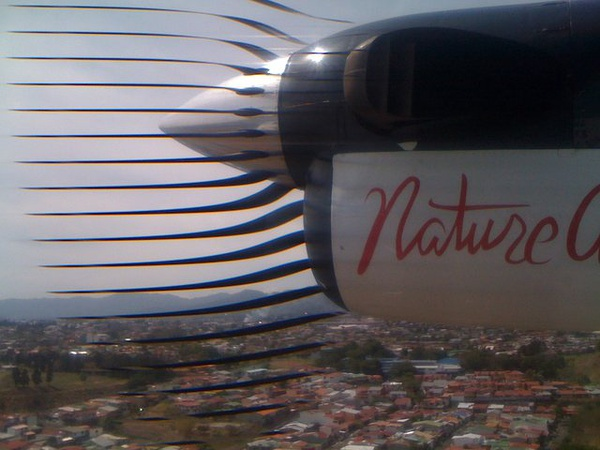
\includegraphics[width=10cm]{jelly}
  \caption{使用卷帘快门摄像头拍摄螺旋桨时产生的果冻效应}
  \label{jelly}
\end{figure}

对于我们的摄像头拍摄时间检测方法来说,当利用LED点阵作为检测信号,使用摄像头对其进行拍摄时,LED点阵中各个LED灯的点亮持续时间较短,变化速度较快,与拍摄的摄像头的卷帘快门打开时间相差较小,因此也会导致果冻效应的产生,影响拍摄结果。典型的果冻效应的图像如图~\ref{jelly2}所示。

\begin{figure}[h] 
  \centering
  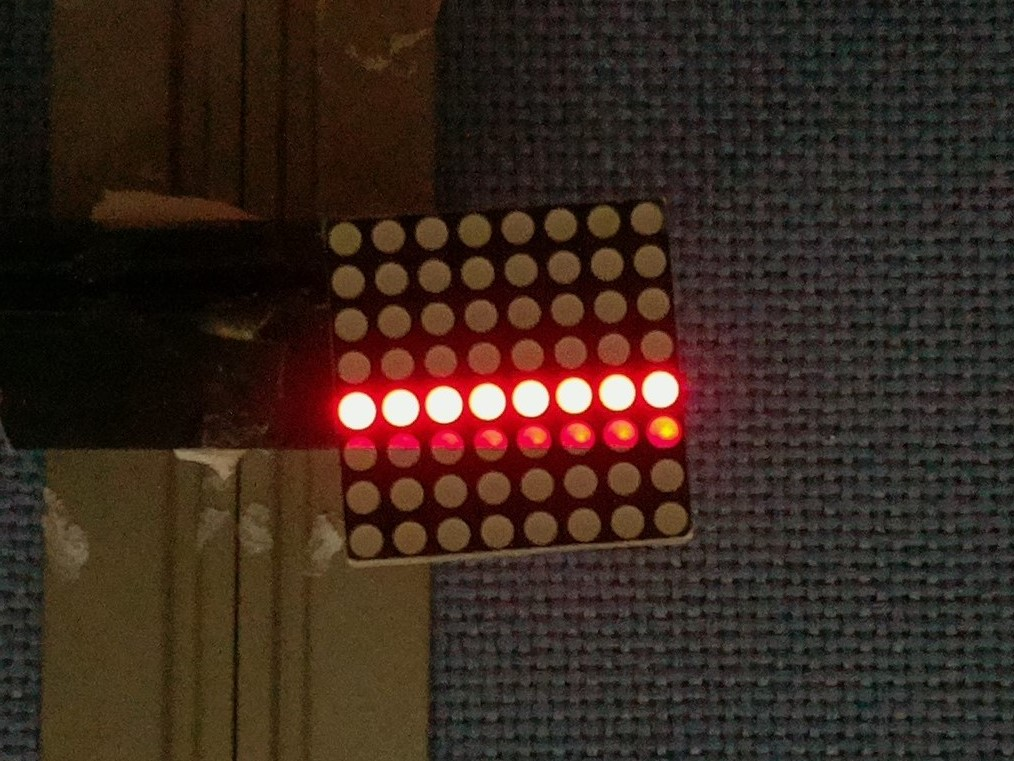
\includegraphics[width=10cm]{jelly2}
  \caption{摄像头拍摄到的果冻效应图像}
  \label{jelly2}
\end{figure}

在该图像中,LED点阵在每个控制周期内点亮一行LED灯,由下至上依次点亮。对于第六行LED灯来说,在摄像头的曝光周期内,与该行LED灯点亮周期的重叠时间较短,因此亮度要低于第五行。观察图像可以发现,在第六行左侧几个LED灯只有半个灯点亮。由于每行LED灯同时点亮且每个LED灯整个灯同时点亮,所以不会出现半个灯点亮的情况,这种现象正是因为摄像头的果冻现象所导致的。当摄像头卷帘快门由上至下依次打开,由于第六行LED灯处于倾斜状态,在曝光开始时第六行的LED灯处于点亮周期末期时,右侧几个LED灯所对应的感光传感器的快门打开时,传感器曝光,拍摄到点亮图像,而左侧几个LED灯所对应的传感器的快门此时尚未打开,所以未拍摄到点亮图像。在很短的时间后,其对应的快门打开时,但是此时LED灯已经熄灭,所以只拍摄到了左侧几个LED灯熄灭的图像。

当利用摄像头拍摄LED点阵图像时。设置LED点阵按照~\ref{flow1}节所介绍的流水编码方法进行变化,控制周期为1ms,即每1ms有一个LED灯熄灭,另一个LED灯点亮,摄像头拍摄的曝光时间长度为5ms。因此,理论上当摄像头开始曝光的时间与LED点阵控制周期开始时间重合时,在摄像头的曝光时间段内共有5个LED灯发生亮灭变化,因为摄像头的拍摄过程是时间积分,光线叠加的过程,所以摄像头能够拍摄到的图像内有5个LED灯被点亮。但是大多数情况下,摄像头开始曝光时间无法与LED点阵控制周期的开始时间精确重合,也就会导致在摄像头的曝光周期内会有多一个,即6个LED灯发生亮灭变化,摄像头拍摄到的图像内会有6个LED灯被点亮,即如图~\ref{take}所示的情况。

\begin{figure}[h] 
  \centering
  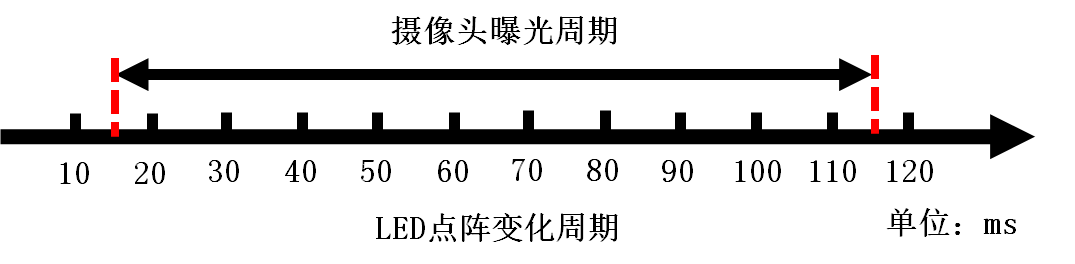
\includegraphics[width=13cm]{take}
  \caption{摄像头曝光时间与LED点阵之间的关系}
  \label{take}
\end{figure}

在实际拍摄过程中,如果在摄像头曝光时间段内,发生变化的LED灯都处于同一行,则如理论推测一样能够拍摄到6个LED灯点亮,如图~\ref{t1}所示。而当发生变化的LED灯不处于同一行时,LED点阵最后一行末尾若干个LED灯发生亮灭变化,然后第一行开始若干个LED灯也发生了亮灭变化,此时摄像头拍摄到的点亮的LED灯数就会少于6个,如图~\ref{t3}所示共有4个LED灯被点亮。这是由于摄像头采用的卷帘快门在拍摄时产生了果冻效应,最后一行LED灯所对应的摄像头的感光传感器的曝光时间,要短于第一行,也要短于摄像头设置的5ms的曝光时间。理论上最后一行倒数第三、四个灯在摄像头曝光周期内也发生了亮灭变化,但在其变化过程中,最后一行所对应的传感器的卷帘快门尚未打开,LED灯的灯光未在传感器上发生光线积分,而当传感器开始曝光时,这两个灯已经熄灭,因此只能拍摄到这两个灯的熄灭状态,总的点亮的LED灯点也就只有4个。

\begin{figure}[h]
  \centering%
  \subcaptionbox{变化的LED灯在同一行内\label{t1}}
    {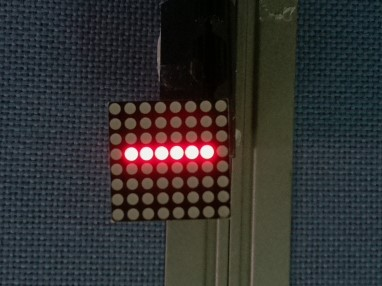
\includegraphics[height=5cm]{t1}}
  \subcaptionbox{变化的LED灯不在同一行内\label{t3}}
      {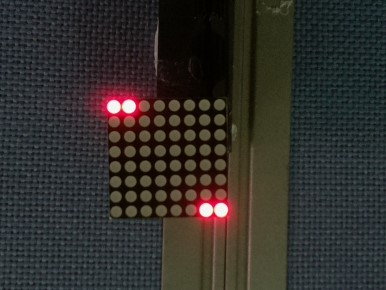
\includegraphics[height=5cm]{t3}}
  \caption{由于果冻效应在相同条件下拍摄到不同数量的LED灯点亮}
  \label{t}
\end{figure}

这种情况是由于摄像头自身硬件性能所导致,由于摄像头卷帘快门的打开时间较长,在拍摄快速变化的LED点阵时会产生果冻效应影响拍摄到的点亮LED灯的数目。而在日常应用中,由于拍摄对象变化较慢,这种现象并不明显。由于果冻效应的影响,使得利用LED点阵检测摄像头拍摄时间时,会对检测结果造成影响,无法准确拍摄拍摄到的LED点阵状态,但是这种硬件层面的问题无法有效解决,因此只能在设计LED点阵编码方法时,避免在一个曝光时间内有多行LED灯发生变化,这样对于逐行曝光的卷帘快门的摄像头,拍摄到的LED灯都处于同一水平位置,能够有效减少果冻效应的影响。

\subsection{多摄像头视野校准}

对于多摄像头系统的应用来说,在实现系统同步的基础之上还有一个重要的问题就是多个摄像头的位置分布,不同的位置分布可以实现不同的系统功能。对于本文所介绍的多摄像头系统,希望实现的一个功能就是利用多个摄像头实现高速摄像,因此也就要求各个摄像头拍摄相同的对象,但是拍摄时间有所差别,然后将各个摄像头拍摄到的图像按照时间顺序穿插起来,以提高摄像帧率。如果拍摄对象在不同摄像头拍摄的图像内处于不同的位置,那么将图像穿插之后拍摄对象的位置发生变化就会造成视频内容的抖动。因此需要在拍摄过程中调整各个摄像头的视野,使得拍摄对象在各个摄像头内处于相同的位置。

为了调整各个摄像头的视野相同,最直接的办法就是利用精密支架进行微调,通过不断比对调整摄像头位置,但是这样的过程费时费力,且调整精度过低。本文提出了一种基于偏振分光棱镜的解决办法,利用不同光路组合有效解决了这个问题。

偏振分光棱镜(Ppolarization Beam splitter,PBS)是一种光学器件,如图~\ref{pbs}所示,它能够将一束入射光分成两束相互垂直的光。如图~\ref{pbs2}所示,当入射光与棱镜胶层成$45^{\circ}$射入偏振分光棱镜时,棱镜能够将入射光分为两束,一束与入射光方向相同,另一束与入射光成$90^{\circ}$,与棱镜胶层成$45^{\circ}$。因此在棱镜的反射光和折射光处各放置一个摄像头,摄像头进行曝光时入射的光线即为同一条光线分成的两束,也就能够保证两个摄像头拍摄到相同的对象,设定各个摄像头视野相同。如果系统内有更多的摄像头,则可以增加偏振分光棱镜的数量,将第一个棱镜分离的两束光线再次进行分离,变为四束光线,以此类推实现系统摄像头数目的扩充。

\begin{figure}[h]
  \centering%
    \subcaptionbox{偏振分光棱镜实物图 \label{pbs}}
    {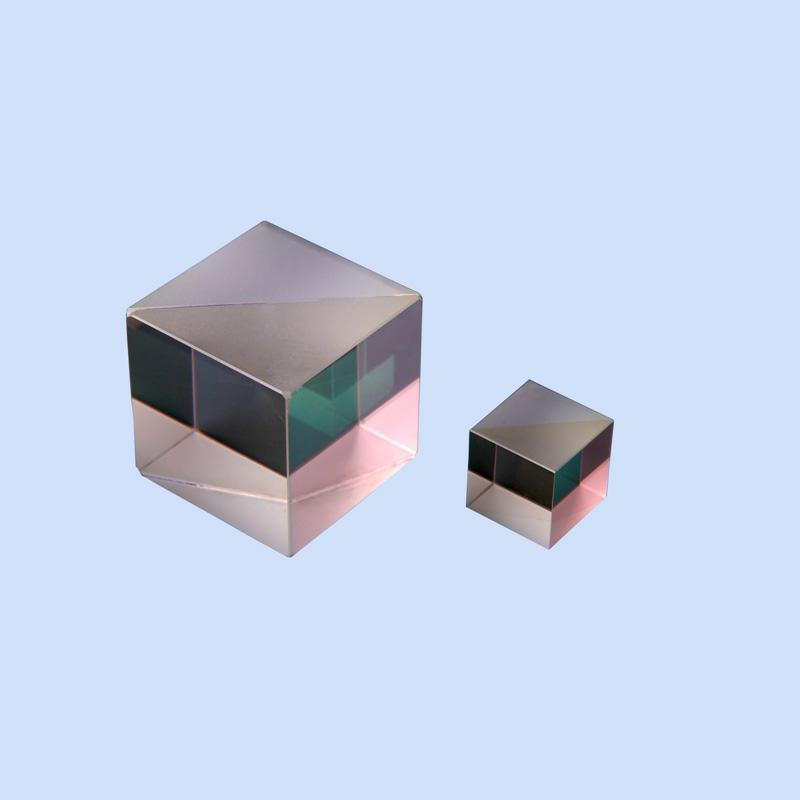
\includegraphics[height=5cm]{pbs}}
  \subcaptionbox{偏振分光棱镜光路\label{pbs2}}
      {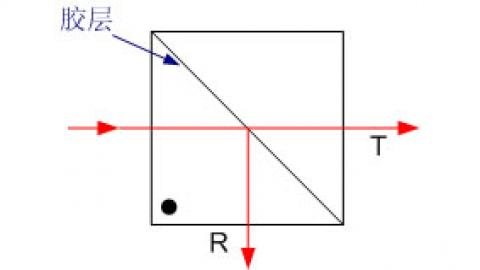
\includegraphics[height=4cm, width=7cm]{pbs2}}
  \caption{偏振分光棱镜}
\end{figure}

为了能够更加方便快捷地使用偏振分光棱镜进行拍摄,本文设计了如下多摄像头视野校准装置。该装置利用三个偏振分光棱镜进行分光,可以使用四个摄像头进行拍摄,棱镜和摄像头利用精密螺丝进行固定并可以调节角度位置,装置外壳可以起到一定的保护作用并屏蔽外界光线对于棱镜分光的影响。装置设计图如图~\ref{eq1}所示,光路图如图~\ref{eq2}所示,实物图如图~\ref{eq3}、~\ref{eq4}所示。

\begin{figure}[h]
  \centering%
    \subcaptionbox{设计图 \label{eq1}}
    {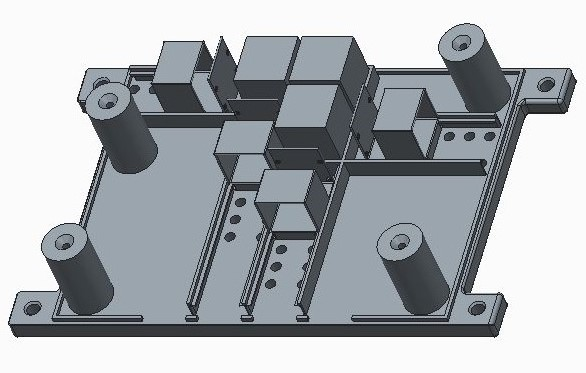
\includegraphics[height=5cm]{eq1}}
  \subcaptionbox{光路图\\.\label{eq2}}
      {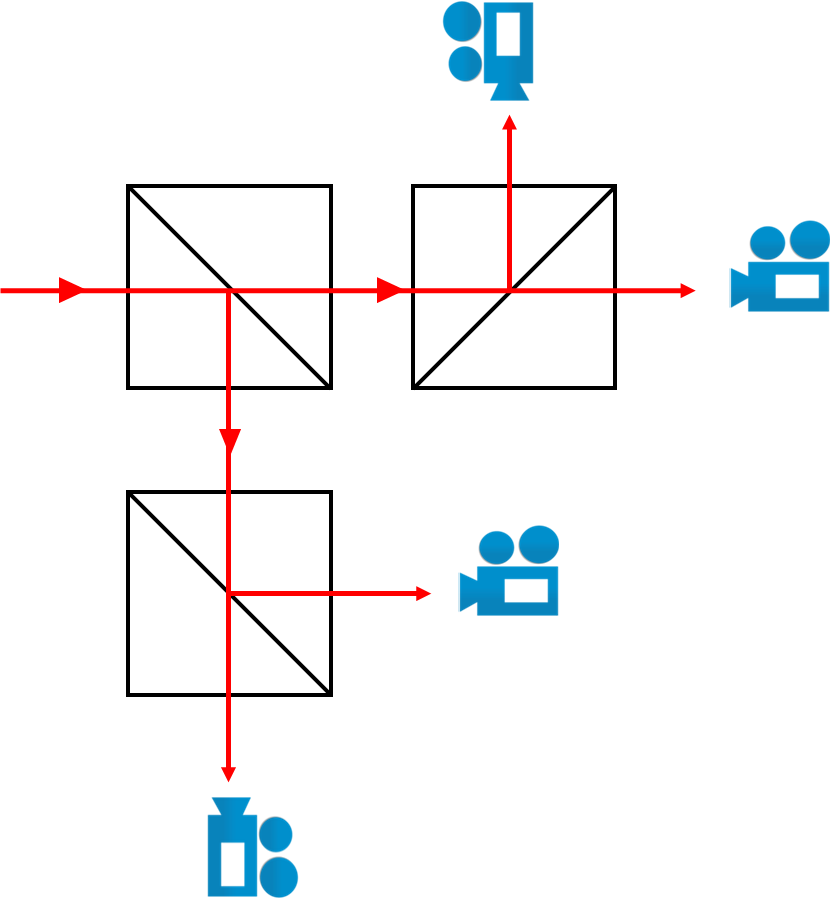
\includegraphics[height=5cm, width=6cm]{eq2}}
  \subcaptionbox{实物图\label{eq3}}
      {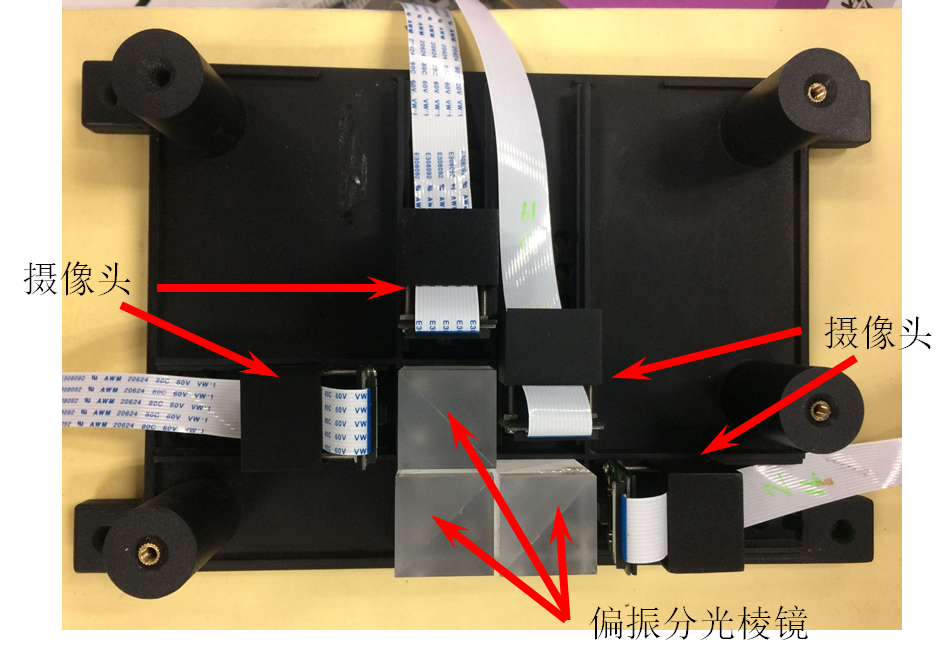
\includegraphics[height=5cm]{eq4}}
  \subcaptionbox{实物图\label{eq4}}
      {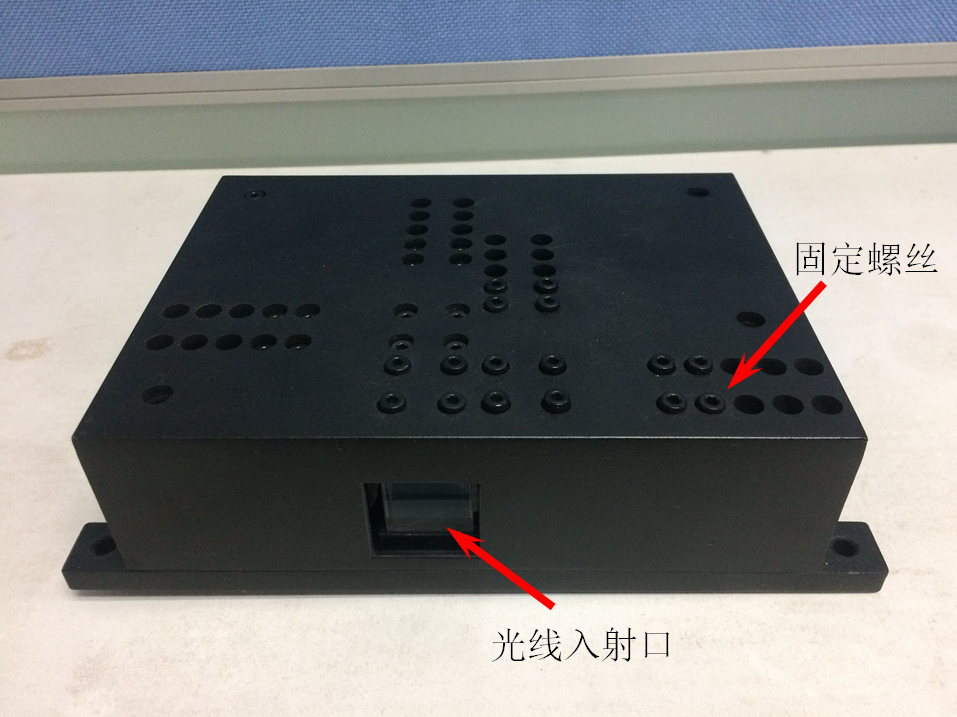
\includegraphics[height=5cm]{eq3}}
  \caption{多摄像头视野校准装置}
\end{figure}

利用该装置进行拍摄时,只需要正确放置偏振分光棱镜的方向,固定好摄像头,并利用固定螺丝调整好摄像头角度即可保证各个摄像头视野相同,拍摄到的图像相同。利用未经同步的四个摄像头进行拍摄,结果如如图~\ref{pbsR}所示。图像边缘是偏振分光棱镜相互之间反射折射光线的结果,可以经过后期处理去掉边缘,中间部分为拍摄对象,且拍摄的视野范围近似相同。由于偏振分光棱镜在分光过程中会降低光线亮度,经过两级分光亮度降低更多,同时由于装置外壳隔绝部分外界光线的射入,以及装置的光线入射口较小,使得各个摄像头拍摄到的图像亮度较低,此问题可以通过增加摄像头曝光时间长度解决。

\begin{figure}[h]
  \centering%
    \subcaptionbox{摄像头一\\.}
    {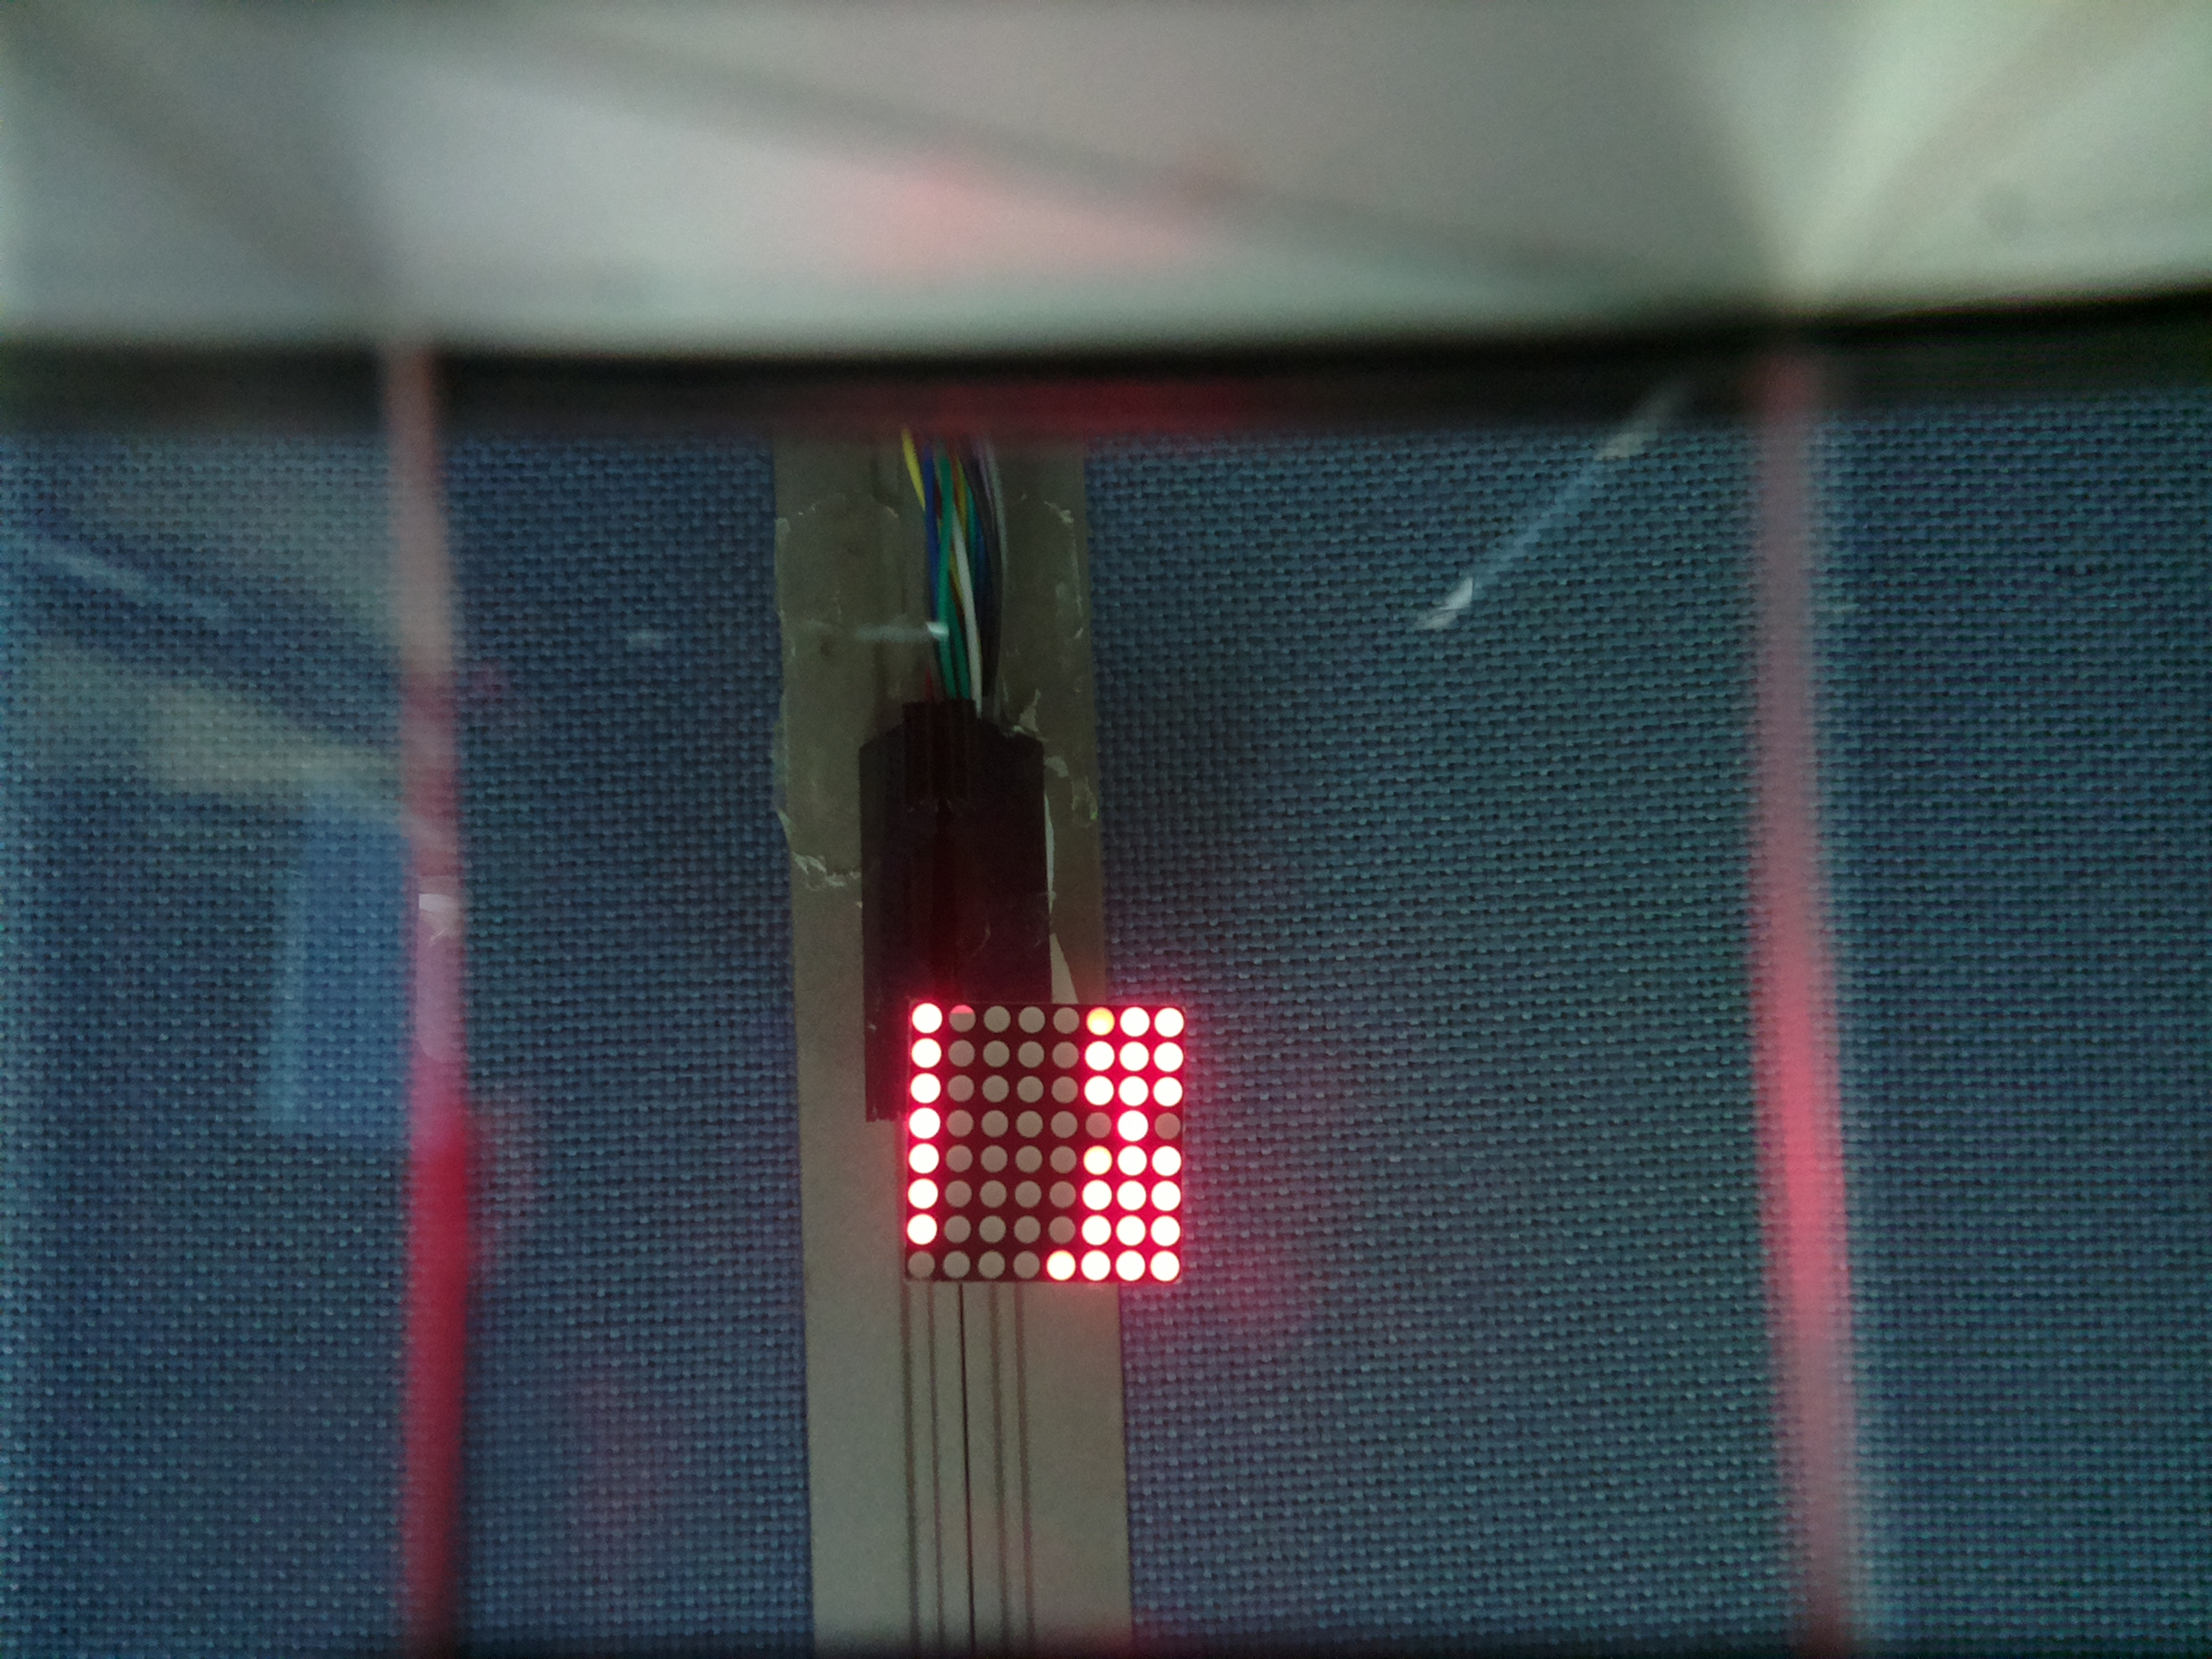
\includegraphics[height=5cm]{pbsR1}}
  \subcaptionbox{摄像头二}
      {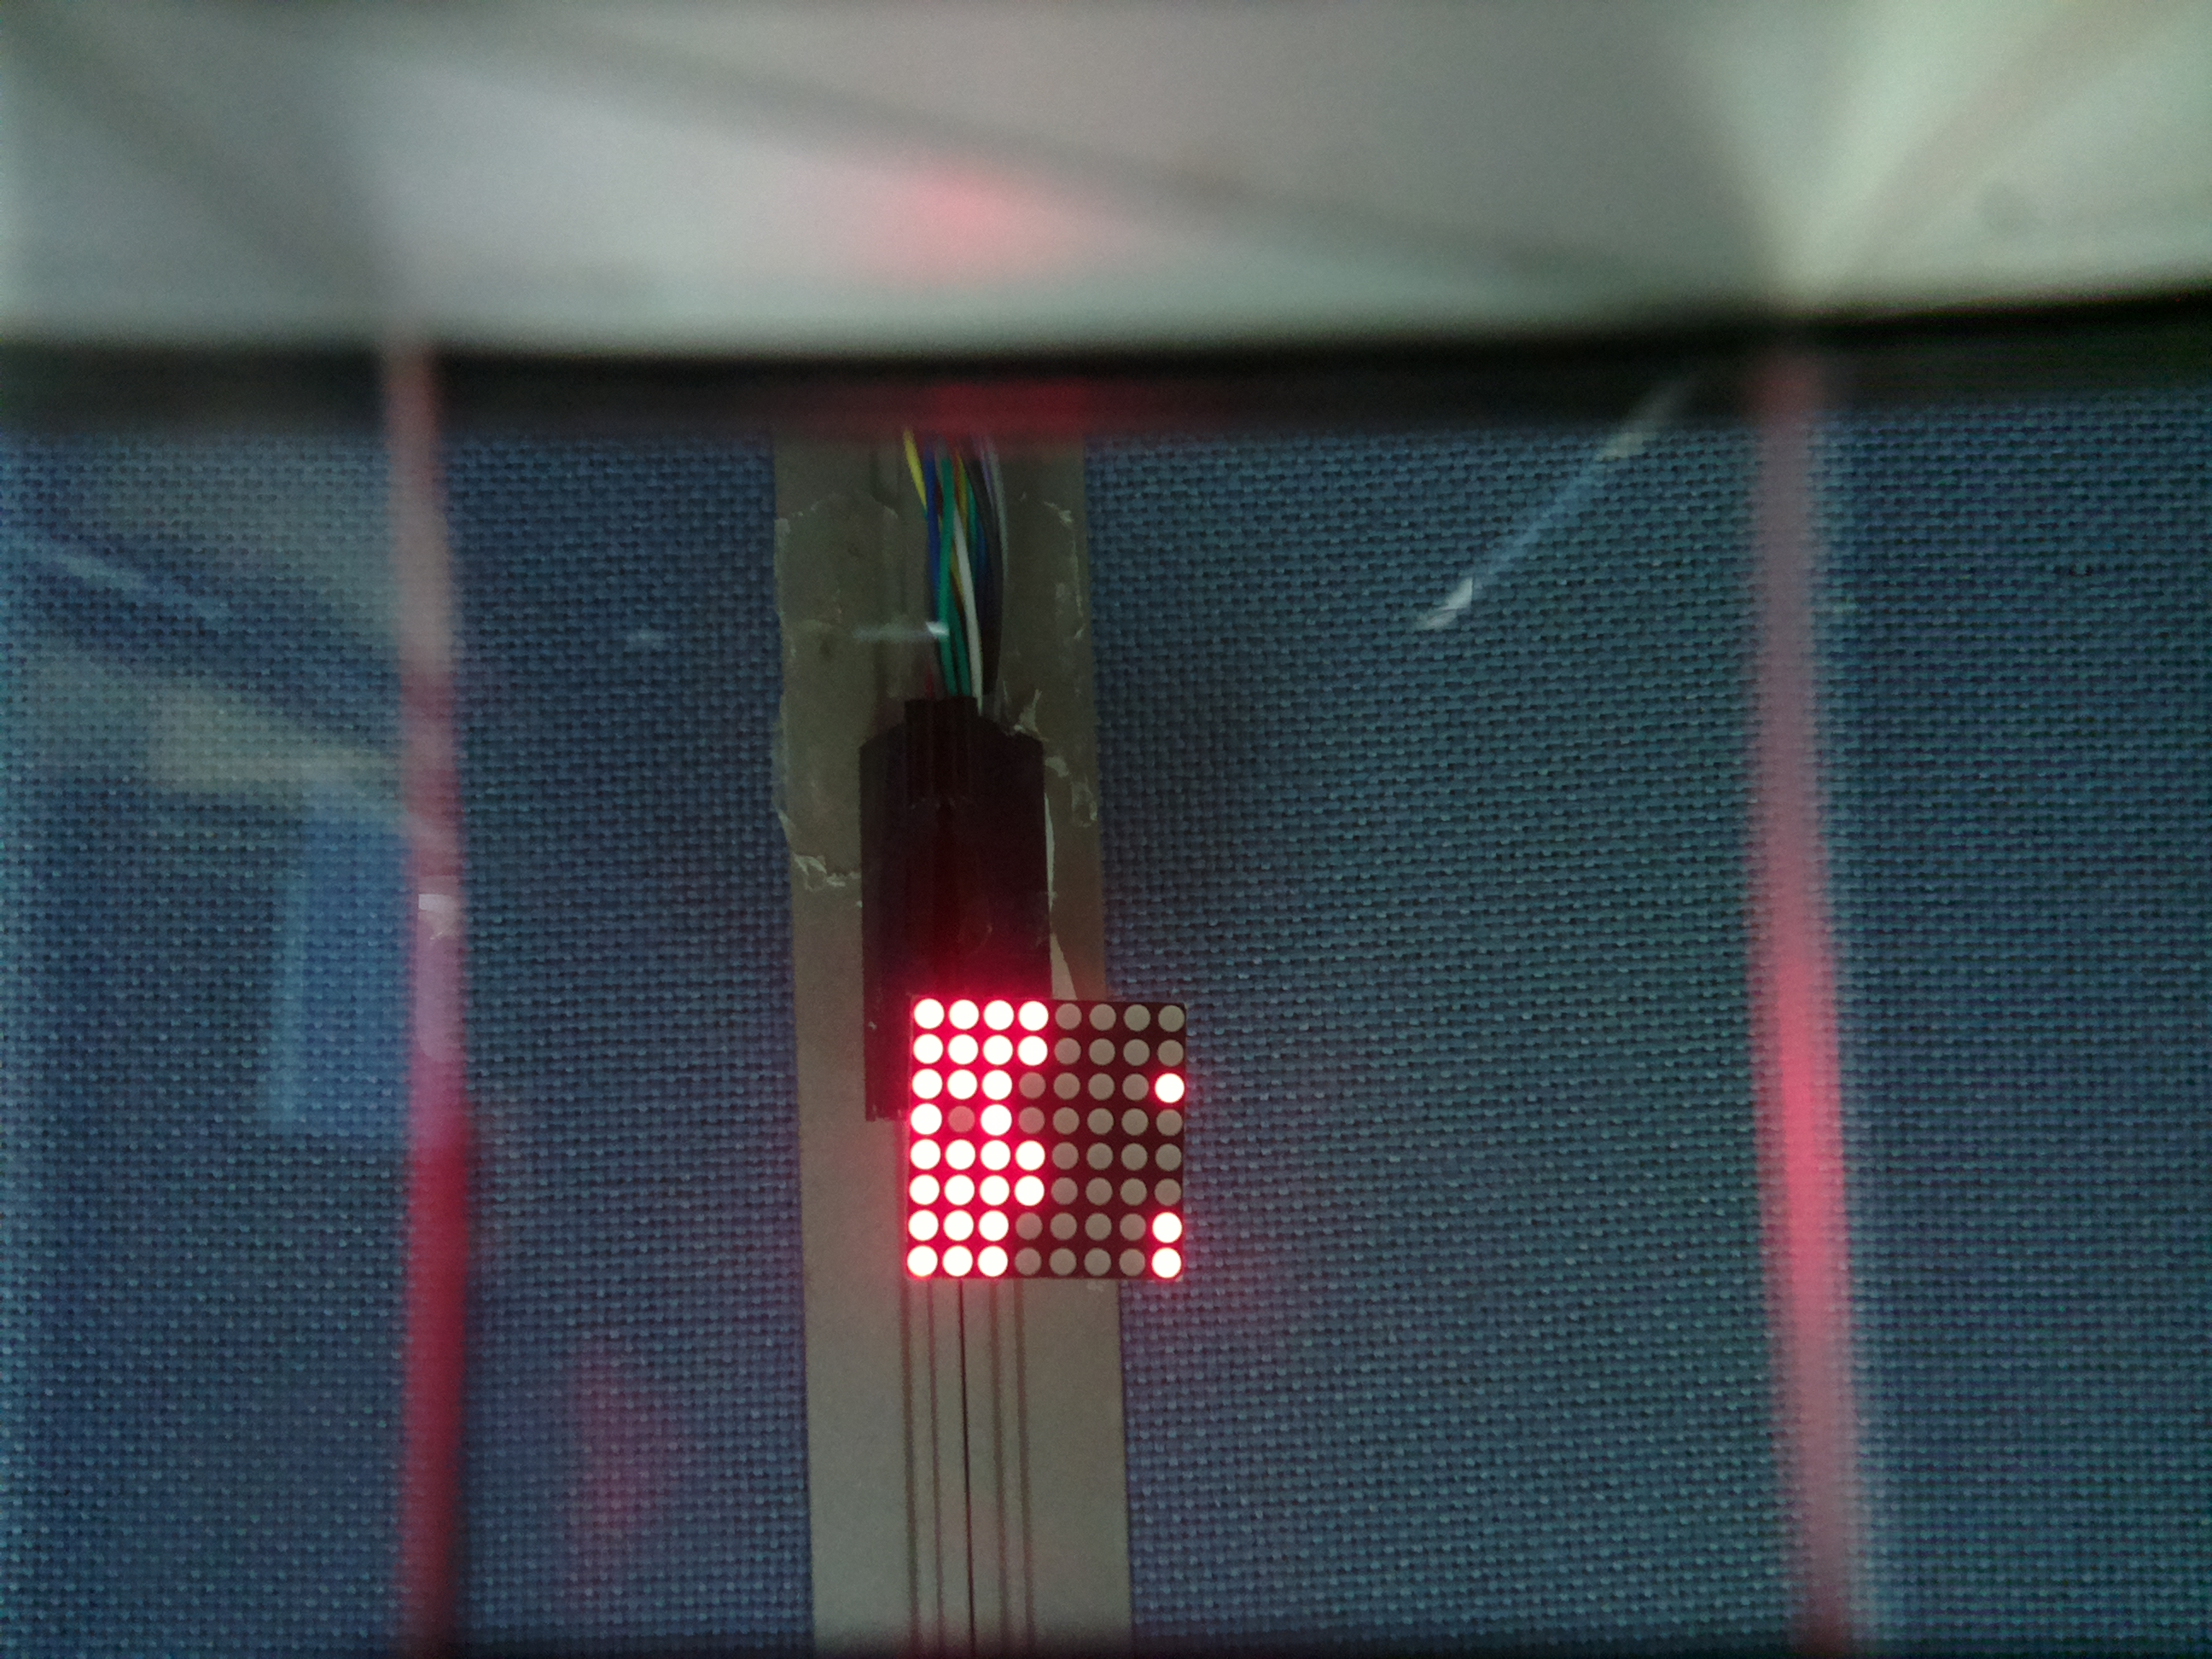
\includegraphics[height=5cm]{pbsR2}}
  \subcaptionbox{摄像头三}
      {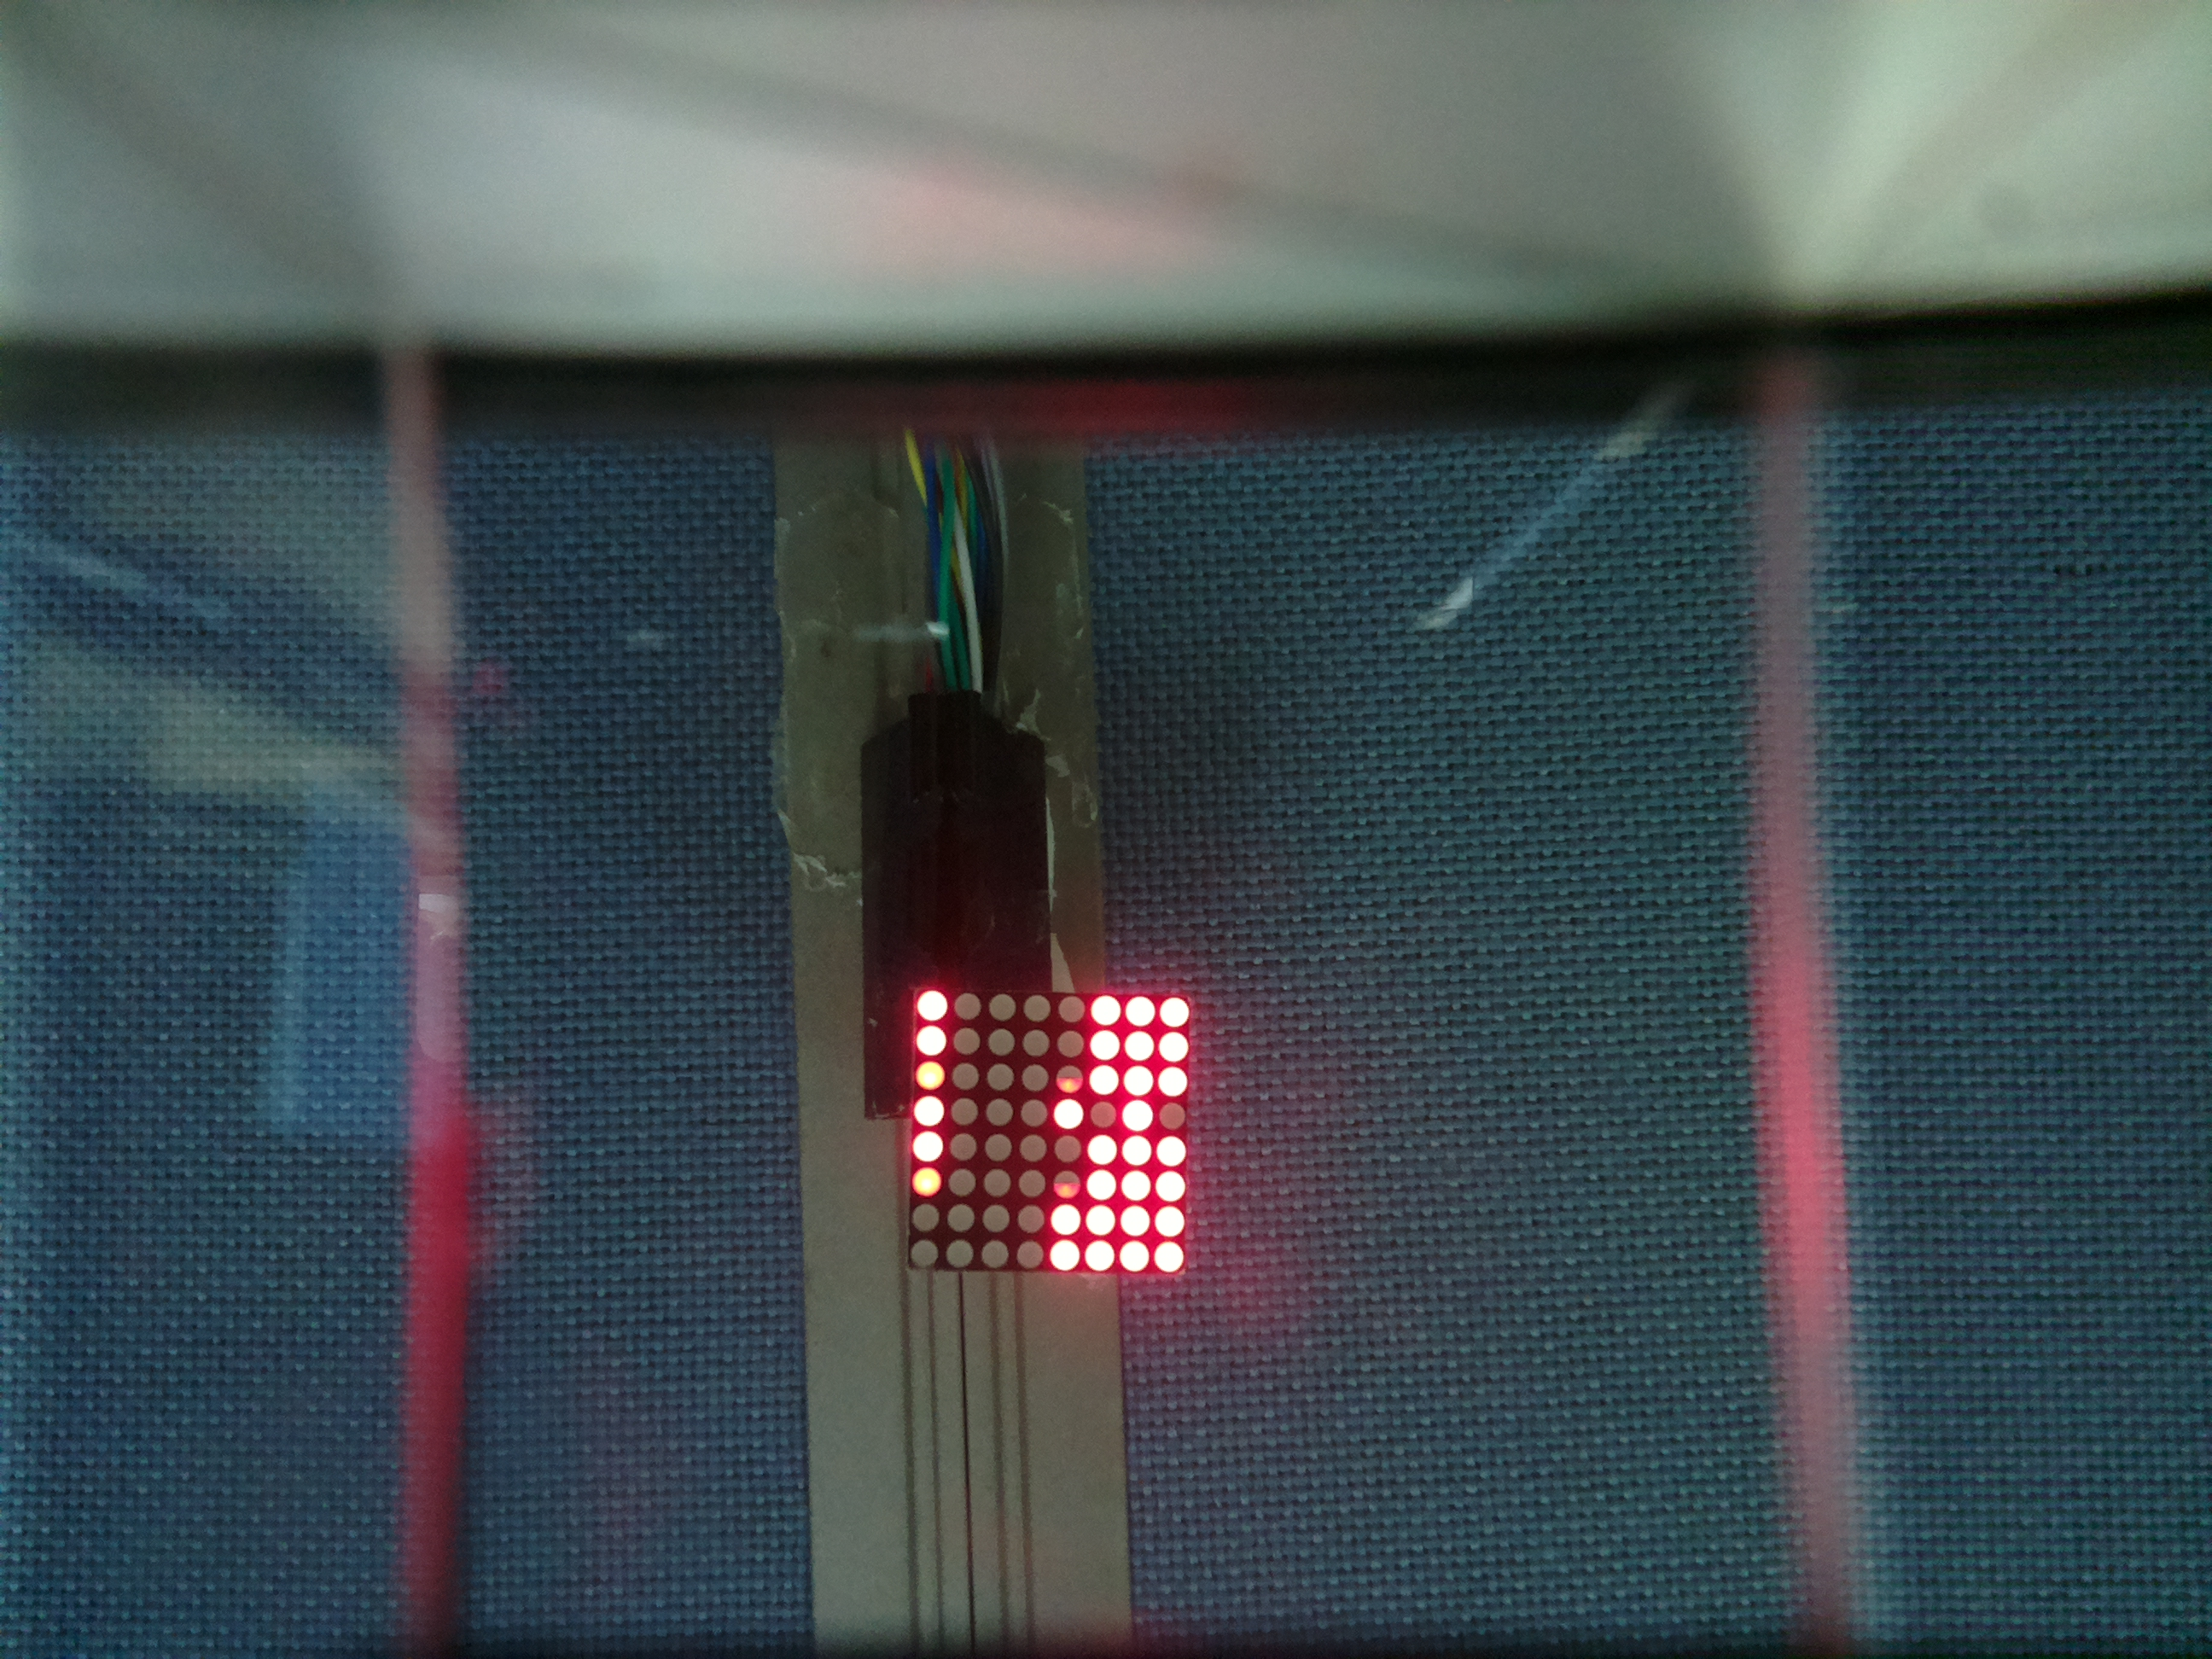
\includegraphics[height=5cm]{pbsR3}}
  \subcaptionbox{摄像头四}
      {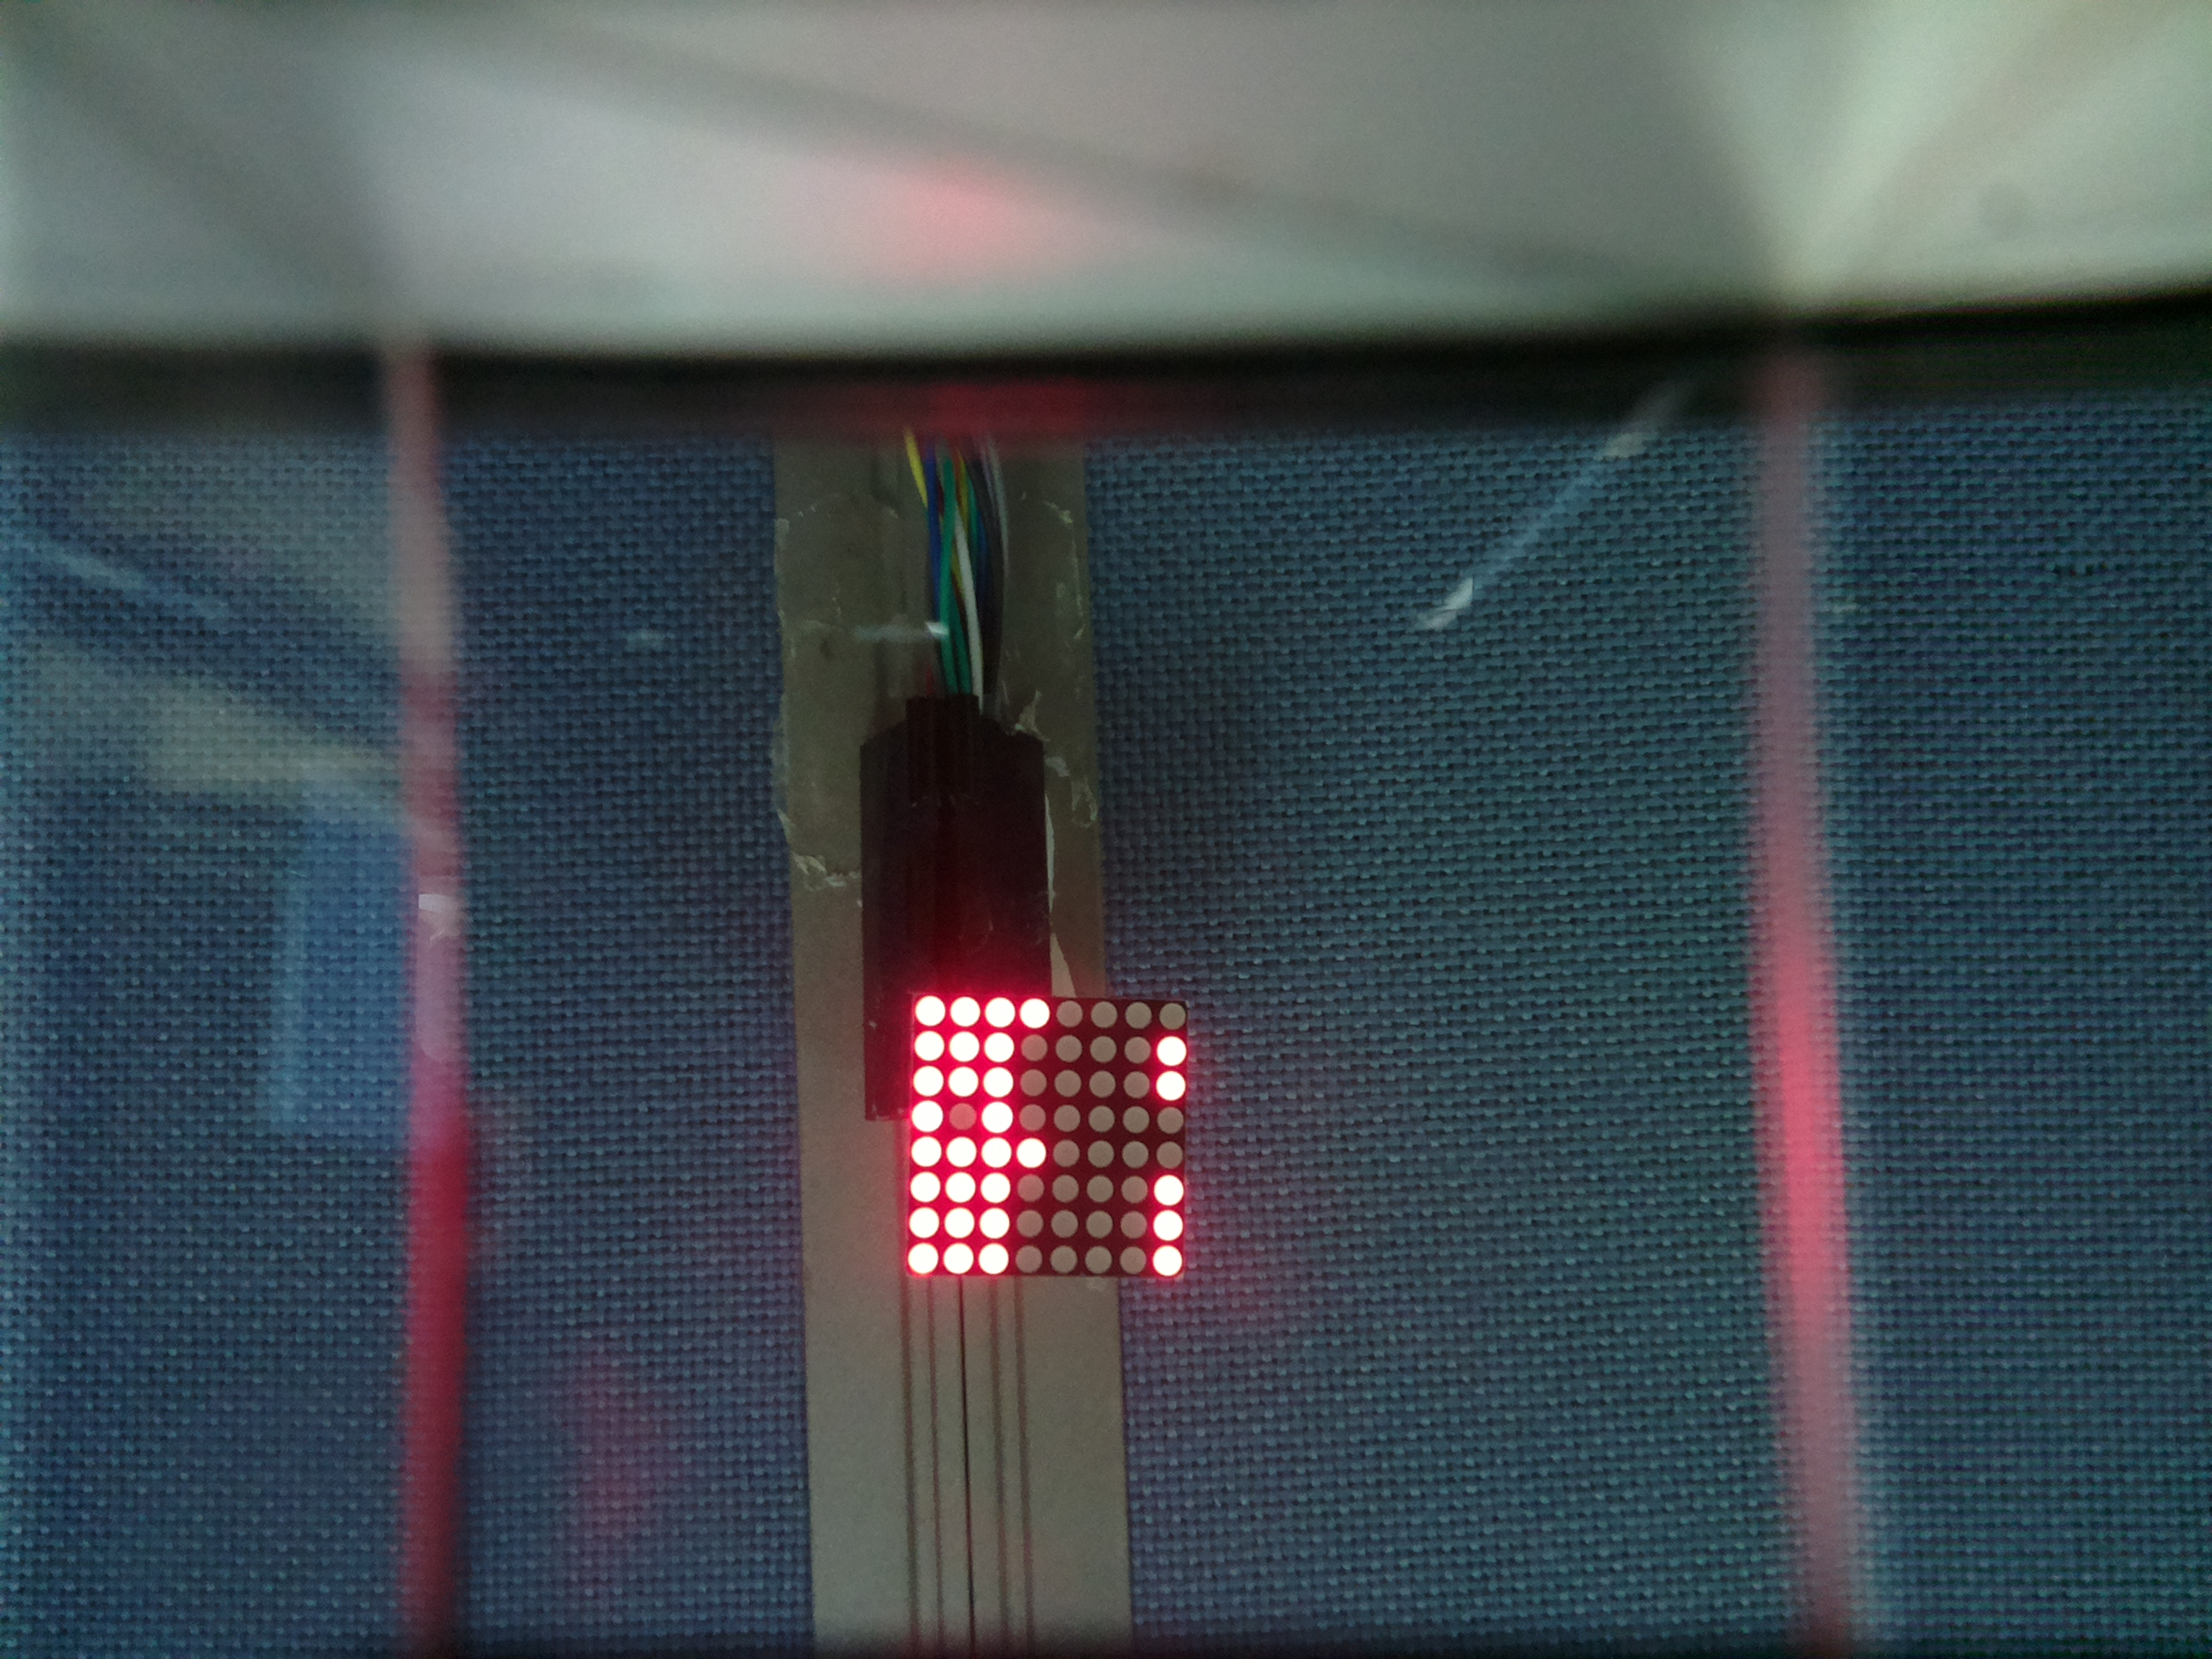
\includegraphics[height=5cm]{pbsR4}}
  \caption{多摄像头拍摄结果}
  \label{pbsR}
\end{figure}

\section{系统同步过程}
\label{proSec}

本节主要介绍多摄像头系统的同步过程。这个过程依赖服务器对各个摄像头的控制,在利用拍摄时间检测系统检测出各个摄像头真实拍摄时间的基础上,通过不断调整各个摄像头的拍摄时间,逐步将系统同步。整个同步过程可分为系统网络通信、检测系统配置、拍摄时间检测、检测结果处理、迭代反馈调整等几个步骤。在同步过程中,只需要配置好图像处理服务器与各个摄像头之间的连接,并设置好检测系统和摄像头的各项参数,在摄像头开始拍摄后将LED点阵放置在摄像头视野范围内,使其能够拍摄到清晰的LED点阵图像,在摄像头正常拍摄的过程中,获取其中一张图像,并将图像传回服务器进行处理,检测各个摄像头的拍摄时间,并经过服务器的计算,向各个摄像头发送控制命令,调整其拍摄时间,之后再次获取LED点阵图像验证调整结果。最终通过多次迭代逐步使系统逼近同步。该同步过程实现简单,同步结果较为精确,能够在摄像头运行过程当中进行同步,且可以保持摄像头设置好的各项工作参数不变,能够适用于多种多摄像头系统。

\textbf{a) 系统网络通信}

本文使用的各个摄像头由独立Linux操作系统分别进行控制,每个操作系统控制一个摄像头。图像处理服务器不外接摄像头,与各个操作系统在同一个局域网内连接,这样可以有效减少信号传输时延。同样,也可以将各个摄像头和服务器都连接到互联网当中,设置成为网络摄像头,也可以实现同步功能。系统结构如图~\ref{system}所示。

\begin{figure}[h] 
  \centering
  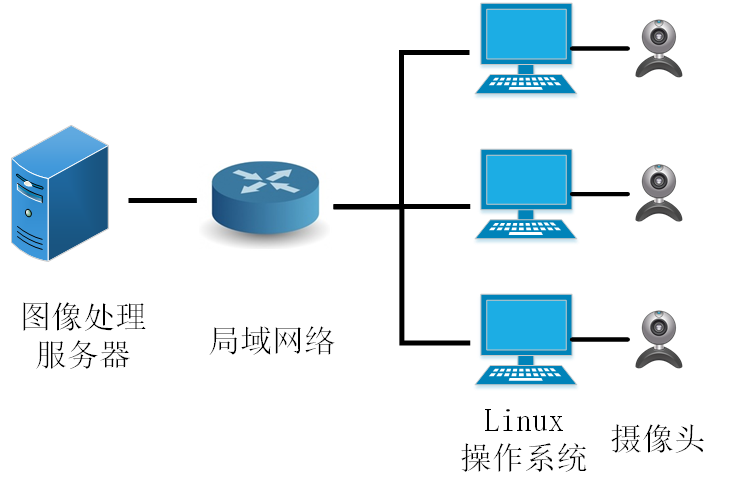
\includegraphics[height=5cm]{system}
  \caption{多摄像头系统结构}
    \label{system}
\end{figure}

在整个系统内,服务器与摄像头之间建立TCP连接,通过套接字(Socket)进行通信。各个摄像头定期向服务器发送心跳信号,确保连接有效。通信数据采用明文传递简单信息,后期还可以进行优化对信息进行加密,并减少数据量。

\textbf{b) 检测系统配置}

根据对同步精度的要求,以及摄像头性能要求,设置检测系统LED点阵的编码方式和控制周期,同时设置摄像头的各项参数,如曝光时间、帧率、图像分辨率等。例如,在采用进位流水方法进行LED点阵编码时,其对于拍摄时间的检测精度如公式~\ref{4}所示,与控制周期有关,因此需要调整LED点阵的控制周期。同时,由于检测过程还与摄像头的曝光时间有关,所以需要先确定摄像头的工作参数,再根据曝光时间设计LED点阵的分组方法,具体设计方法在~\ref{flowSe}节已经有所介绍。当设置好LED点阵和摄像头的参数后,还要根据各项设置修改图像处理服务器同步程序内图像检测参数和摄像头控制参数,以便能够检测出拍摄到的LED点阵状态,并计算各个摄像头之间的拍摄时间差,并进行调整。

另外,检测的过程中,需要将LED点阵置于摄像头的拍摄范围内,使得摄像头能够拍摄到清晰、完整的LED点阵的图像。因此,需要根据各个摄像头的拍摄视角,选取合适的距离和角度,放置好LED点阵,以提高同步精度。而当同步结束之后,或者不需要进行同步的时候,可以将LED点阵移出系统拍摄范围,不影响系统的正常工作。

\textbf{c) 拍摄时间检测}

对于多摄像头系统的同步过程是在系统正常运行,摄像头正常进行拍摄的过程当中完成的,而且为了实现同步,各个摄像头的拍摄帧率必然相同,所以各个摄像头拍摄到的每帧图像之间的时间差是保持不变的。如图~\ref{sequence}所示,各个摄像头两帧之间的时间差相同,开始进行拍摄后,不同摄像头之间的拍摄时间差保持不变,且差值小于单一摄像头相邻两帧之间的时间间隔。

\begin{figure}[h] 
  \centering
  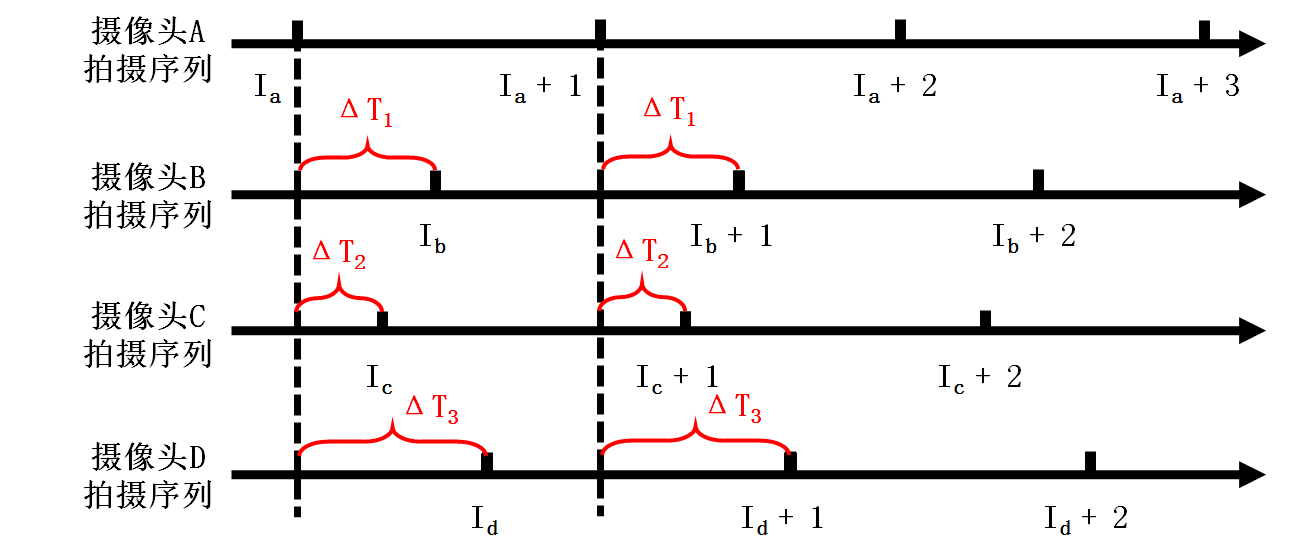
\includegraphics[height=5cm]{sequence}
  \caption{多摄像头拍摄时间序列}
    \label{sequence}
\end{figure}

当需要进行时间同步时,首先需要检测各个摄像头的拍摄时间。在设置好LED点阵的位置后,图像服务器会向各个摄像头发送获取图像的命令,将摄像头拍摄到的LED点阵图像保存,此时拍摄到的点阵状态代表了摄像头的拍摄时间。

保存图像结束后,各个摄像头会将拍摄到的图像传回图像服务器进行处理。由于对于整个同步过程的耗时长度并没有特殊要求,因此并不要求各个摄像头在保存结束后立即回传图像,以免发生网络拥塞。在服务器得到所有摄像头拍摄图像后,根据~\ref{detecSe}节所介绍的方法对于摄像头的拍摄时间进行检测。虽然服务器向各个摄像头发送命令要求其同时进行,但是由于控制信息网络传输延时、系统延时、硬件延时等多种原因,各个摄像头的真实拍摄时间可能会有所不同,得到的LED点阵的状态也就不同,服务器通过检测图像获得的各个摄像头的拍摄时间自然也就不同。

在这个拍摄时间检测过程中,服务器向各个摄像头发送拍摄命令是依次进行发送,要求摄像头在接收到命令后立即进行拍摄。虽然对于运算速率较快的服务器程序运行速度较快,命令发送过程持续的时间长度较短,可以认为是同在同一时间进行发送。同时,由于服务器与摄像头处于同一个局域网络内,控制信息的网络传输时间也较短,传输时间可以忽略不计。但是服务器信号发送过程有可能因为系统内部运行而出现延时,当服务器与摄像头通过互联网连接,网络传输存在延时时,各个摄像头就无法再同一时间接收到控制信号。

因此,为了进一步提高同步精度,在以上检测方法的基础之上还可以采用另一种改进的方法,即利用网络时间协议(Network Time Protocol,NTP)协议将图像服务器与控制摄像头的Linux操作系统进行系统时间同步。将图像服务器同时设置成为NTP服务器,在Linux操作系统上运行NTP服务,在局域网络内利用NTP协议将图像服务器与控制摄像头的操作系统的系统时间首先进行同步。然后当服务器需要控制摄像头进行拍摄收,向各个摄像头发送命令要求摄像头在未来的某一时刻开始进行拍摄,此时即使服务器发送命令或者网络信号传输存在延时,只要能够保证在要求拍摄的时刻之前摄像头接收到控制信号即可,这些延时并不会影响控制结果。

\textbf{d) 检测结果处理}

在服务器计算出各个摄像头的拍摄时间之后,服务器选取其中一个摄像头作为同步基准,其他摄像头与这个摄像头的拍摄时间差即为系统的同步误差。为了尽可能缩小系统误差,使得同步过程更快,在选取基准摄像头时,根据所有摄像头的拍摄时间顺序进行排列,选取拍摄时间居中的摄像头作为基准,能够使得系统总的同步误差绝对值最小。

在选取好基准摄像头,获得其他摄像头与其的拍摄时间差后,服务器会发送命令,控制其他摄像头调整拍摄时间。具体的调整方法有两种,一是使摄像头停止拍摄,暂停一段时间后重新启动拍摄,如果重新启动的时间与基准摄像头的拍摄时间相同,则能够达到同步目的。其中,暂停的时间取决于检测到的拍摄时间差,如果被检测摄像头的拍摄时间早于基准摄像头$T$时间,则需要将被调整摄像头暂停$T + n * t_{int}$时间,其中$t_{int}$表示摄像头拍摄两帧图像之间的时间差,即帧率的倒数,$n$为任意自然数,用来增大暂停的时间间隔。如果被检测摄像头的拍摄时间晚于基准摄像头$T$时间,则需要将被调整摄像头暂停$t_{int} - T + n * t_{int}$时间。同时,由于从摄像头接收到控制命令,到完成停止拍摄和开始拍摄的操作之间,存在信号传输延时、操作系统运行延时、硬件延时等延时,在计算暂停时间时需要将这些延时加入到其中。

第二种方法不需要关闭摄像头,在摄像头拍摄过程当中改变摄像头的帧率,并在新的帧率下运行一段时间,由于在这段时间内该摄像头与基准摄像头的帧率不同,各帧的拍摄时间差也就会随之发生变化。在运行一段时间后,再将摄像头的帧率调整回正常工作的帧率,即可使两摄像头拍摄时间相同。假如被调整摄像头与基准摄像头之间拍摄时间差为$T$,调整前帧率和调整后帧率分别为$f_1, f_2$,则调整前后摄像头拍摄两帧之间的时间间隔分别为$1/f_1, 1/f_2$,则在不同帧率下拍摄的每帧的时间差经过多帧积累即可补齐两个摄像头之间总的时间差,而为了避免总时间差过短,新帧率运行时间也随之过短,可以将总时间差增加$n$个每帧拍摄时间间隔,因此新帧率的运行时间$T$如公式~\ref{adj}所示:

\begin{equation}
T = \left\{
\begin{aligned}
&\frac {f_1*T + n}{|f_1- f_2|} & \text{(拍摄时间早于基准摄像头)}\\
&\frac {1- f_1*T + n}{|f_1- f_2|}  &\text{(拍摄时间晚于基准摄像头)}
\end{aligned}
\right.
  \label{adj}
\end{equation}

同样,在采取该方法时,也需要考虑到系统内存在的延时,将该延时加入到新帧率运行时长当中。

\textbf{e) 迭代反馈调整}

通过多次实验可知,该对摄像头进行调整时,系统内存在的各项延时并不固定,该时间间隔在一定范围内小幅度波动,因此从开始进行同步调整到调整结束,这一过程所经历的时间是不确定的,与程序设定的时间间隔有一定的随机误差。因此,在进行同步调整之后,还要进一步验证调整结果,即重复以上第三和第四步,再次检测系统内是否仍存在不同步的摄像头,然后对其进行调整,直至所有摄像头都能够在同一时间拍摄,实现系统同步。

\section{本章小结}

本章主要介绍了对多摄像头系统进行时间同步的主要过程。在该过程当中存在的果冻效应问题是卷帘快门自身的硬件性能所致,在对高速运动物体进行拍摄时会加剧该效应,因此会对高精度的拍摄时间检测造成影响,为了消除此影响,需要在检测方法的设计和LED点阵编码方法设计过程中考虑该问题,消除果冻效应的影响。而多摄像头的视野校准问题则通过精细调整可以解决,但耗时耗力稳定性不强,利用本文提出的方法能够有效解决该问题,且具有可扩展性、可调节性和一定的稳定性。本章还介绍了系统同步的具体方法,该方法能够对多摄像头系统内各摄像头分别进行调节,且该调节过程可以在系统正常运行过程当中进行,对系统性能无过多要求,具有一定的普适性,还可以根据需求设置不同的同步精度,具有一定的灵活性。但该方法存在的问题在于由于系统内随机延时的影响,会导致调节结果与预想结果不符,需要经过多次迭代不断提高调节准确性。




















































































